\documentclass[a4paper,twoside]{article}
\usepackage{blindtext}  
\usepackage{geometry}

% Chinese support
\usepackage[UTF8, scheme = plain]{ctex}

% Page margin layout
\geometry{left=2.3cm,right=2cm,top=2.5cm,bottom=2.0cm}


\usepackage{listings}
\usepackage{xcolor}
\usepackage{geometry}
\usepackage{amsmath}
\usepackage{float}
\usepackage{hyperref}

\usepackage{graphics}
\usepackage{graphicx}
\usepackage{subcaption}
\usepackage{epsfig}
\usepackage{float}

\usepackage{algorithm}
\usepackage[noend]{algpseudocode}

\usepackage{booktabs}
\usepackage{threeparttable}
\usepackage{longtable}
\usepackage{tikz}
\usepackage{multicol}
\usepackage{pgfplots}
\pgfplotsset{compat=1.9}
\pgfplotsset{
    myplotstyle/.style={
    legend style={draw=none, font=\small},
    legend cell align=left,
    legend pos=north east,
    ylabel style={align=center, font=\bfseries\boldmath},
    xlabel style={align=center, font=\bfseries\boldmath},
    x tick label style={font=\bfseries\boldmath},
    y tick label style={font=\bfseries\boldmath},
    scaled ticks=false,
    every axis plot/.append style={thick},
    },
}

% cite package, to clean up citations in the main text. Do not remove.
\usepackage{cite}

\usepackage{color,xcolor}

%% The amssymb package provides various useful mathematical symbols
\usepackage{amssymb}
%% The amsthm package provides extended theorem environments
\usepackage{amsthm}
\usepackage{amsfonts}
\usepackage{enumerate}
\usepackage{enumitem}
\usepackage{listings}
\usepackage{minted}


\usepackage{indentfirst}
\setlength{\parindent}{2em} % Make two letter space in the first paragraph
\usepackage{setspace}
\linespread{1.5} % Line spacing setting
\usepackage{siunitx}
\setlength{\parskip}{0.5em} % Paragraph spacing setting

% \usepackage[contents =22920202204622, scale = 10, color = black, angle = 50, opacity = .10]{background}

\renewcommand{\figurename}{图}
\renewcommand{\listingscaption}{代码}
\renewcommand{\tablename}{表格}
\renewcommand{\contentsname}{目录}
\floatname{algorithm}{算法}

\graphicspath{ {images/} }

%%%%%%%%%%%%%
\newcommand{\StudentNumber}{22920202204622}  % Fill your student number here
\newcommand{\StudentName}{熊恪峥}  % Replace your name here
\newcommand{\PaperTitle}{实验(二)}  % Change your paper title here
\newcommand{\PaperType}{实验报告} % Replace the type of your report here
\newcommand{\Date}{2023年4月3日}
\newcommand{\College}{信息学院}
\newcommand{\CourseName}{数据库}
%%%%%%%%%%%%%

%% Page header and footer setting
\usepackage{fancyhdr}
\usepackage{lastpage}
\pagestyle{fancy}
\fancyhf{}
% This requires the document to be twoside
\fancyhead[LO]{\texttt{\StudentName }}
\fancyhead[LE]{\texttt{\StudentNumber}}
\fancyhead[C]{\texttt{\PaperTitle }}
\fancyhead[R]{\texttt{第{\thepage}页,共\pageref*{LastPage}页}}


\title{\PaperTitle}
\author{\StudentName}
\date{\Date}

\algnewcommand\algorithmicinput{\textbf{Input:}}
\algnewcommand\algorithmicoutput{\textbf{Output:}}
\algnewcommand\Input{\item[\algorithmicinput]}%
\algnewcommand\Output{\item[\algorithmicoutput]}%

\usetikzlibrary{positioning, shapes.geometric}

\begin{document}
	
%%%%%%%%%%%%%%%%%%%%%%%%%%%%%%%%%%%%%%%%%%%%
\makeatletter % change default title style
\renewcommand*\maketitle{%
	\begin{center} 
		\bfseries  % title 
		{\LARGE \@title \par}  % LARGE typesetting
		\vskip 1em  %  margin 1em
		{\global\let\author\@empty}  % no author information
		{\global\let\date\@empty}  % no date
		\thispagestyle{empty}   %  empty page style
	\end{center}%
	\setcounter{footnote}{0}%
}
\makeatother
%%%%%%%%%%%%%%%%%%%%%%%%%%%%%%%%%%%%%%%%%%%%
	
	
\thispagestyle{empty}

\vspace*{1cm}

\begin{figure}[htb]
	\centering
	
\includegraphics[width=4.0cm]{logo.png}
\end{figure}

\vspace*{1cm}

\begin{center}
	\Huge{\textbf{\PaperType}}
	
	\Large{\PaperTitle}
\end{center}

\vspace*{1cm}

\begin{table}[h]
	\centering	
	\begin{Large}
		\renewcommand{\arraystretch}{1.5}
		\begin{tabular}{p{3cm} p{5cm}<{\centering}}
			姓\qquad 名 & \StudentName  \\
			\hline
			学\qquad号 & \StudentNumber \\
			\hline
			日\qquad期 & \Date  \\
			\hline
			学\qquad院 & \College  \\
			\hline
			课程名称 & \CourseName  \\
			\hline
		\end{tabular}
	\end{Large}
\end{table}

\newpage

\title{
	\Large{\textcolor{black}{\PaperTitle}}
}
	
	
\maketitle
	
\tableofcontents
 
\newpage
\setcounter{page}{1}

\begin{spacing}{1.2}

\section{实验2.1}

\begin{enumerate}
\item 查询年级为2001的所有学生的名称并按编号升序排列。
\begin{quote}
\texttt{
select * from STUDENTS where grade=2001 order by sid asc
}
\end{quote}

\begin{figure}[h]
\centering
\caption{运行结果}
\begin{subfigure}{0.3\textwidth}
  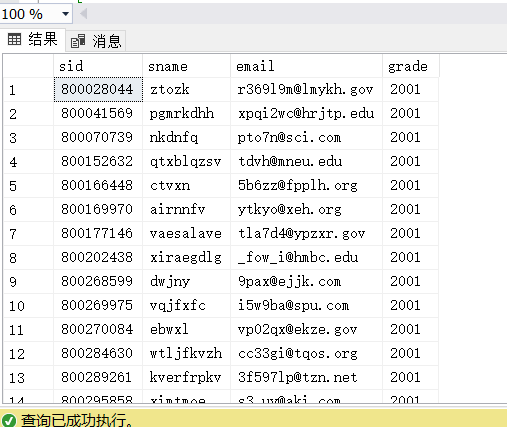
\includegraphics[width=0.9\textwidth]{fig1.png}
\end{subfigure}
\begin{subfigure}{0.3\textwidth}
  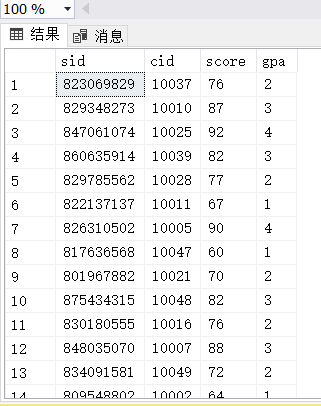
\includegraphics[width=0.9\textwidth]{fig2.png}
\end{subfigure}
\end{figure}

\item 查询学生的选课成绩合格的课程成绩,并把成绩换算为积点(60分对应积点为1,每增加1分,积点增加0.1)。

思路:使用\texttt{CASE}语句分情况讨论,将60一下映射为0,60以上映射为(score-50)/10,即1-5。
\begin{quote}
\texttt{
SELECT sid, cid, score, 
       CASE WHEN score >= 60 THEN (score - 50) / 10 ELSE 0 END AS gpa
FROM CHOICES
WHERE score >= 60;
}
\end{quote}


\begin{figure}[h]
\centering
\caption{运行结果}
\begin{subfigure}{0.3\textwidth}
  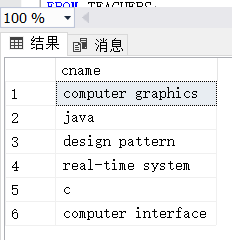
\includegraphics[width=0.9\textwidth]{fig3.png}
\end{subfigure}
\begin{subfigure}{0.3\textwidth}
  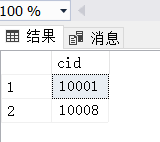
\includegraphics[width=0.9\textwidth]{fig4.png}
\end{subfigure}
\end{figure}


\item 查询课时是48或64的课程的名称。
\begin{quote}
\texttt{
SELECT cname
FROM COURSES
WHERE hour IN (48, 64);
}
\end{quote}


\begin{figure}[h]
\centering
\caption{运行结果}
\begin{subfigure}{0.3\textwidth}
  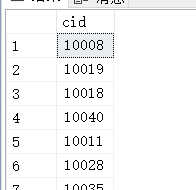
\includegraphics[width=0.9\textwidth]{fig5.png}
\end{subfigure}
\begin{subfigure}{0.3\textwidth}
  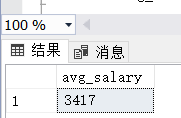
\includegraphics[width=0.9\textwidth]{fig6.png}
\end{subfigure}
\end{figure}


\item 查询所有课程名称中含有data的课程编号。

思路:使用通配符\texttt{\%},表示任意多个字符。
\begin{quote}
\texttt{
SELECT cid
FROM COURSES
WHERE cname LIKE '\%data\%';
}
\end{quote}


\begin{figure}[h]
\centering
\caption{运行结果}
\begin{subfigure}{0.3\textwidth}
  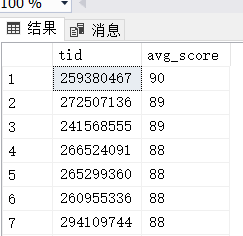
\includegraphics[width=0.9\textwidth]{fig7.png}
\end{subfigure}
\begin{subfigure}{0.3\textwidth}
  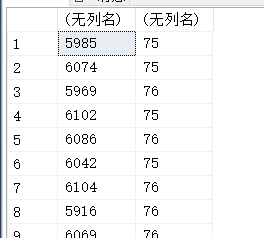
\includegraphics[width=0.9\textwidth]{fig8.png}
\end{subfigure}
\end{figure}


\item 查询所有选课记录的课程号(不重复显示)。
\begin{quote}
\texttt{
SELECT DISTINCT cid
FROM CHOICES;
}
\end{quote}



\item 统计所有教师的平均工资。
\begin{quote}
\texttt{
SELECT AVG(salary) AS avg\_salary
FROM TEACHERS;
}
\end{quote}


\item 查询所有教师的编号及选修其课程的学生的平均成绩,按平均成绩降序排列。
\begin{quote}
\texttt{
SELECT TEACHERS.tid, AVG(CHOICES.score) AS avg\_score
FROM TEACHERS
JOIN CHOICES ON TEACHERS.tid = CHOICES.tid
JOIN STUDENTS ON STUDENTS.sid = CHOICES.sid
GROUP BY TEACHERS.tid
ORDER BY avg\_score desc
}
\end{quote}


\begin{figure}[h]
\centering
\caption{运行结果}
\begin{subfigure}{0.3\textwidth}
  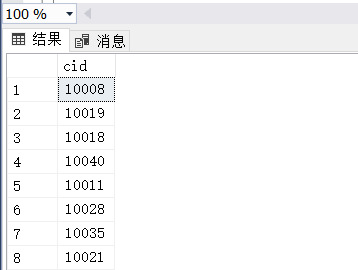
\includegraphics[width=0.9\textwidth]{fig13.png}
\end{subfigure}
\begin{subfigure}{0.3\textwidth}
  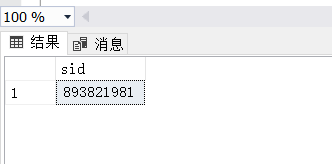
\includegraphics[width=0.9\textwidth]{fig14.png}
\end{subfigure}
\end{figure}


\item 统计各个课程的选课人数和平均成绩。
\begin{quote}
\texttt{
SELECT COUNT(*),AVG(CHOICES.score) from CHOICES
GROUP BY cid
}
\end{quote}


\begin{figure}[h]
\centering
\caption{运行结果}
\begin{subfigure}{0.3\textwidth}
  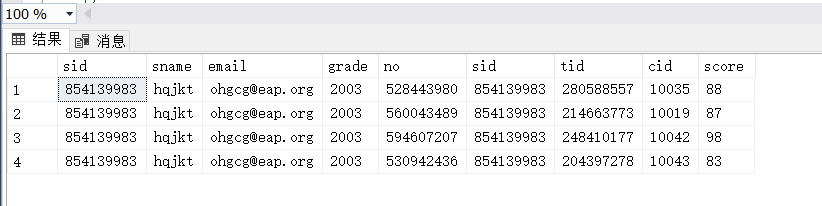
\includegraphics[width=0.9\textwidth]{fig15.png}
\end{subfigure}
\begin{subfigure}{0.3\textwidth}
  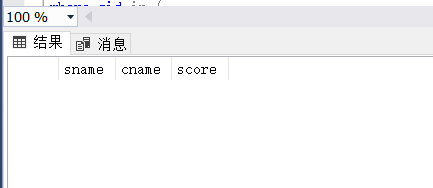
\includegraphics[width=0.9\textwidth]{fig16.png}
\end{subfigure}
\end{figure}


\item 查询至少选修了三门课程的学生编号。
\begin{quote}
\texttt{
SELECT sid from CHOICES
GROUP BY sid
HAVING COUNT(*)>=3
select * from CHOICES where sid=812917218 
}
\end{quote}


\item 查询编号800009026的学生所选的全部课程的课程名和成绩。
\begin{quote}
\texttt{
SELECT cname,score FROM CHOICES JOIN COURSES ON CHOICES.cid = COURSES.cid
where sid = 800009026
}
\end{quote}

\begin{figure}[h]
\centering
\caption{运行结果}
\begin{subfigure}{0.3\textwidth}
  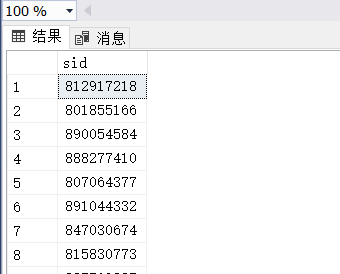
\includegraphics[width=0.9\textwidth]{fig9.png}
\end{subfigure}
\begin{subfigure}{0.3\textwidth}
  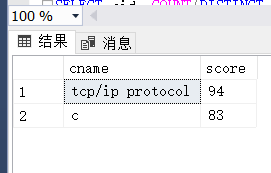
\includegraphics[width=0.9\textwidth]{fig10.png}
\end{subfigure}
\end{figure}


\item 查询所有选修了database的学生的编号。
\begin{quote}
\texttt{
SELECT sid FROM CHOICES where cid in (select cid from COURSES where cname like 'database')
select * from CHOICES where sid=870899566  
select * from COURSES
}
\end{quote}


\begin{figure}[h]
\centering
\caption{运行结果}
\begin{subfigure}{0.3\textwidth}
  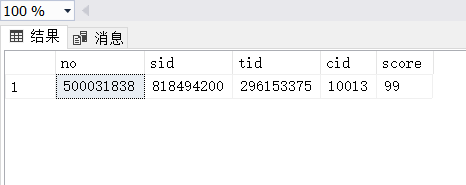
\includegraphics[width=0.9\textwidth]{fig21.png}
\end{subfigure}
\begin{subfigure}{0.3\textwidth}
  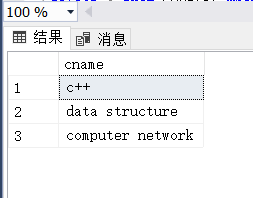
\includegraphics[width=0.9\textwidth]{fig22.png}
\end{subfigure}
\end{figure}


\item 求出选择了同一个课程的学生数。
\begin{quote}
\texttt{
SELECT cid, COUNT(DISTINCT sid) AS num\_of\_students
FROM CHOICES
GROUP BY cid;
}
\end{quote}

\begin{quote}
\texttt{
SELECT COUNT(DISTINCT c1.sid) AS num\_of\_students, c1.cid
FROM CHOICES c1
INNER JOIN CHOICES c2 ON c1.cid = c2.cid AND c1.sid <> c2.sid
GROUP BY c1.cid;
}
\end{quote}

\item 求出至少被两名学生选修的课程编号。
\begin{quote}
\texttt{
SELECT cid FROM CHOICES 
GROUP BY cid
HAVING COUNT(*)>=2
select * from CHOICES where cid=10008
}
\end{quote}


\item 查询选修了编号800009026的学生所选的某个课程的学生编号。
\begin{quote}
\texttt{
select top(1) sid from CHOICES
where cid in (
	select cid from CHOICES where sid = 800009026
)
order by NEWID()
}
\end{quote}
\item 查询学生的基本信息及选修课程编号和成绩。
\begin{quote}
\texttt{
select * from STUDENTS JOIN CHOICES \\
ON STUDENTS.sid = CHOICES.sid 
where STUDENTS.sid=854139983
}
\end{quote}


\begin{figure}[h]
\centering
\caption{运行结果}
\begin{subfigure}{0.3\textwidth}
  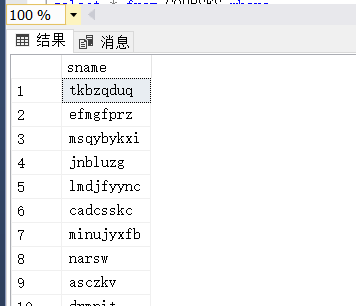
\includegraphics[width=0.9\textwidth]{fig23.png}
\end{subfigure}
\begin{subfigure}{0.3\textwidth}
  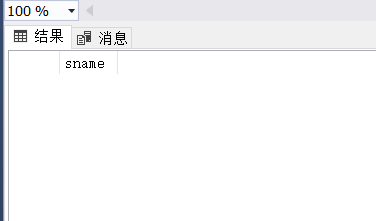
\includegraphics[width=0.9\textwidth]{fig24.png}
\end{subfigure}
\end{figure}


\item 查询学号850955252的学生的姓名和选修的课程名及成绩。
\begin{quote}
\texttt{
SELECT s.sname, c.cname, ch.score
FROM STUDENTS s, CHOICES ch, COURSES c
WHERE s.sid = ch.sid AND ch.cid = c.cid AND s.sid = '850955252';
}
\end{quote}
\item 查询与学号850955252的学生同年级的所有学生资料。
\begin{quote}
\texttt{
SELECT * FROM STUDENTS 
where grade in (SELECT grade from STUDENTS where sid='850955252')
}
\end{quote}

\begin{figure}[h]
\centering
\caption{运行结果}
\begin{subfigure}{0.3\textwidth}
  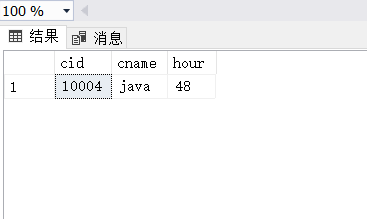
\includegraphics[width=0.9\textwidth]{fig19.png}
\end{subfigure}
\begin{subfigure}{0.3\textwidth}
  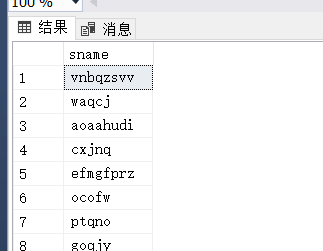
\includegraphics[width=0.9\textwidth]{fig20.png}
\end{subfigure}
\end{figure}

\item 查询所有有选课的学生的详细信息。
\begin{quote}
\texttt{
select * from STUDENTS 
where sid in (
select distinct sid from CHOICES
)
}
\end{quote}
\item 查询没有学生选的课程的编号。
\begin{quote}
\texttt{
select * from COURSES
where cid not in (
select distinct cid from CHOICES
)
}
\end{quote}

\begin{figure}[h]
\centering
\caption{运行结果}
\begin{subfigure}{0.3\textwidth}
  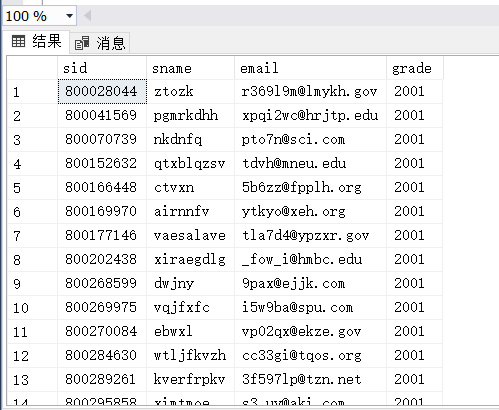
\includegraphics[width=0.9\textwidth]{fig17.png}
\end{subfigure}
\begin{subfigure}{0.3\textwidth}
  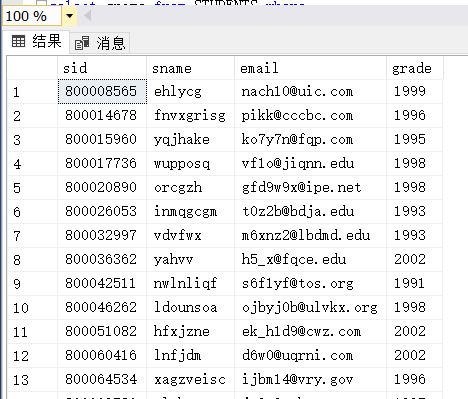
\includegraphics[width=0.9\textwidth]{fig18.png}
\end{subfigure}
\end{figure}


\item 查询选修了与C++的课时一样课程的学生名称。
\begin{quote}
\texttt{
select sname from STUDENTS where
sid in (
select distinct sid from CHOICES where cid in (
select distinct cid from COURSES where hour in (
select hour from COURSES where cname like 'c++'
)
)
)
}
\end{quote}


\item 找出选修课程成绩最好的选课记录。
\begin{quote}
\texttt{
select top (1) * from CHOICES
order by score DESC
}
\end{quote}
\item 找出和课程UML或课程C++的课时一样课程名称。
\begin{quote}
\texttt{
select cname from COURSES where hour in (
select hour from COURSES where cname like 'C++' or cname like 'UML'
)
}
\end{quote}


\begin{figure}[h]
\centering
\caption{运行结果}
\begin{subfigure}{0.3\textwidth}
  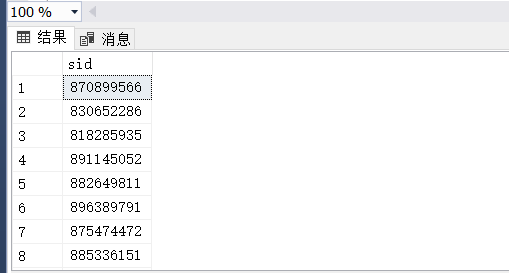
\includegraphics[width=0.9\textwidth]{fig11.png}
\end{subfigure}
\begin{subfigure}{0.3\textwidth}
  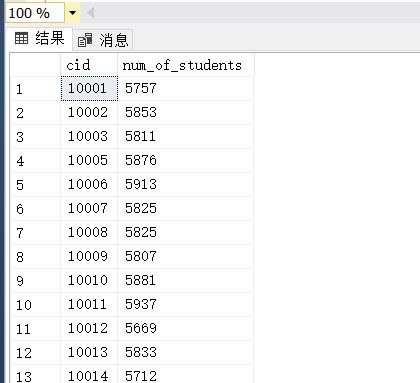
\includegraphics[width=0.9\textwidth]{fig12.png}
\end{subfigure}
\end{figure}

\item 查询所有选修编号10001的课程的学生的姓名。
\begin{quote}
\texttt{
select sname from STUDENTS where sid in(
select distinct sid from CHOICES where cid = 10001
)
}
\end{quote}
\item 查询选修了所有课程的学生姓名。
\begin{quote}

思路一、查询条件“为不存在一门课程,该学生没选”

思路二、查询学生不同的选课ID数量和COURSE表中课程数量相等的学生

两种做法如下:

\texttt{
SELECT sid from CHOICES 
where not exists(
select * from COURSES where
cid not in (select CHOICES.cid from CHOICES where CHOICES.sid = sid)
)
}
\end{quote}
\begin{quote}
\texttt{
SELECT sname
FROM STUDENTS
WHERE sid IN (
  SELECT sid
  FROM CHOICES
  GROUP BY sid
  HAVING COUNT(DISTINCT cid) = (
    SELECT COUNT(*) FROM COURSES
  )
);
}
\end{quote}

\begin{figure}[h]
\centering
\caption{运行结果}
\begin{subfigure}{0.3\textwidth}
  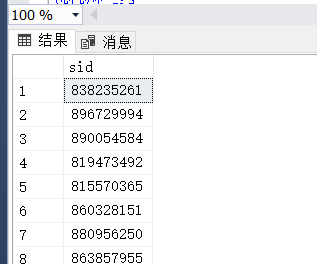
\includegraphics[width=0.9\textwidth]{fig25.png}
\end{subfigure}
\begin{subfigure}{0.3\textwidth}
  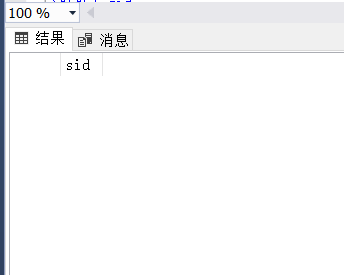
\includegraphics[width=0.9\textwidth]{fig26.png}
\end{subfigure}
\end{figure}

\item 利用集合运算,查询选修课程C++或选修课程Java的学生的编号。
\begin{quote}
\texttt{
SELECT sid
FROM CHOICES
WHERE cid = (SELECT cid FROM COURSES WHERE cname = 'C++')
UNION
SELECT sid
FROM CHOICES
WHERE cid = (SELECT cid FROM COURSES WHERE cname = 'Java');
}
\end{quote}
\item 实现集合交运算,查询既选修课程C++又选修课程Java的学生的编号。
\begin{quote}
\texttt{
SELECT sid
FROM CHOICES
WHERE cid = (SELECT cid FROM COURSES WHERE cname = 'C++')
INTERSECT
SELECT sid
FROM CHOICES
WHERE cid = (SELECT cid FROM COURSES WHERE cname = 'Java');
}
\end{quote}
\item 实现集合减运算,查询选修课程C++而没有选修课程Java的学生的编号。
\begin{quote}
\texttt{
SELECT sid
FROM CHOICES
WHERE cid = (SELECT cid FROM COURSES WHERE cname = 'C++')
EXCEPT
SELECT sid
FROM CHOICES
WHERE cid = (SELECT cid FROM COURSES WHERE cname = 'Java');
}
\end{quote}

\begin{figure}[h]
\centering
\caption{运行结果}
\begin{subfigure}{0.3\textwidth}
  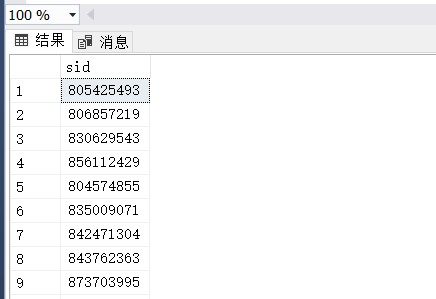
\includegraphics[width=0.9\textwidth]{fig27.png}
\end{subfigure}
\end{figure}

\end{enumerate}

\clearpage

\section{实验2.2}

\begin{enumerate}
\item 查询所有选课记录的成绩并将它换算为五分制(满分5分,合格3分),注意SCORE取NULL值的情况。

思路:使用CASE WHEN THEN END语句处理NULL,将其替换成0

\begin{quote}
\texttt{
SELECT no, sid, tid, cid,
  CASE 
    WHEN score IS NULL THEN NULL
    WHEN score >= 60 THEN (score-60)/10+2
    ELSE 0.0
  END AS gpa
FROM CHOICES;
}
\end{quote}
\item 通过查询选修编号10028的课程的学生的人数,其中成绩合格的学生人数,不合格的学生人数,讨论NULL值的特殊含义。
\begin{quote}
\texttt{
SELECT 
  COUNT(*) AS total\_students,
  SUM(CASE WHEN score IS NULL THEN 0 ELSE 1 END) AS scored\_students,
  SUM(CASE WHEN score >= 60 THEN 1 ELSE 0 END) AS passed\_students,
  SUM(CASE WHEN score >= 60 THEN 0 WHEN score IS NULL THEN 0 ELSE 1 END) AS failed\_students
FROM CHOICES
WHERE cid = '10028';
}
\end{quote}

在这道题的条件下,NULL值的含义可能是缺考、缓考等特殊情况导致的没有成绩。


\begin{figure}[h]
  \centering
  \caption{运行结果}
  \begin{subfigure}{0.3\textwidth}
    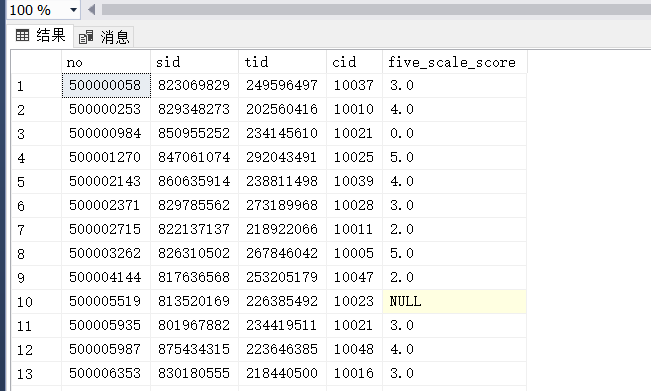
\includegraphics[width=0.9\textwidth]{fig28.png}
  \end{subfigure}
  \begin{subfigure}{0.3\textwidth}
    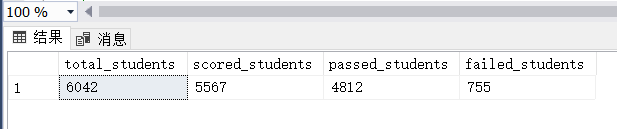
\includegraphics[width=0.9\textwidth]{fig29.png}
  \end{subfigure}
\end{figure}

\item 通过实验检验在使用ORDER BY进行排序时,取NULL的项是否出现在结果中?如果有,在什么位置?
\begin{quote}
\texttt{
SELECT score FROM CHOICES ORDER BY score ASC;
}
\end{quote}

运行以上代码,可以发现ASC排序时最先出现,DESC排序时会最后出现

\item 在上面的查询过程中如果加上保留字DISTINCT会有什么效果?
\begin{quote}
\texttt{
SELECT DISTINCT score FROM CHOICES ORDER BY  score ASC;
}
\end{quote}

运行以上代码,可以发现会保留一个NULL值的项。

\begin{figure}[h]
\centering
\caption{运行结果}
\begin{subfigure}{0.3\textwidth}
  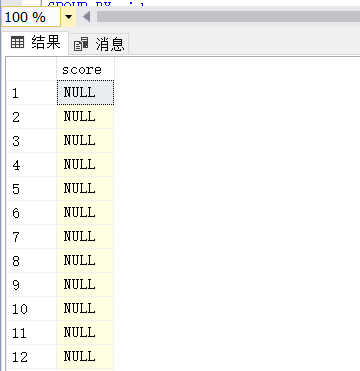
\includegraphics[width=0.9\textwidth]{fig30.png}
\end{subfigure}
\begin{subfigure}{0.3\textwidth}
  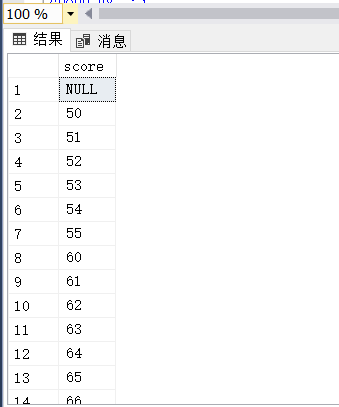
\includegraphics[width=0.9\textwidth]{fig31.png}
\end{subfigure}
\end{figure}

\item 通过实验说明使用分组GROUP BY对取值为NULL的项的处理。
\begin{quote}
\texttt{
SELECT score, COUNT(*) FROM CHOICES GROUP BY score;
}
\end{quote}

会将NULL值的元组单独放在一组中。

\item 结合分组,使用集合函数求每个同学的平均分、总的选课记录数、最高成绩、最低成绩和总成绩。
\begin{quote}
\texttt{
SELECT sid, AVG(score) AS avg\_score, COUNT(*) AS total\_records, MAX(score) AS max\_score, MIN(score) AS min\_score, SUM(score) AS sum\_score
FROM CHOICES
GROUP BY sid;
}
\end{quote}

如果考虑NULL,可以将其替换成0。函数ISNULL可以将NULL值替换成0。

\begin{quote}
\texttt{
SELECT sid, AVG(ISNULL(score, 0)) AS avg\_score, COUNT(*) AS total\_records, MAX(ISNULL(score, 0)) AS max\_score, MIN(ISNULL(score, 0)) AS min\_score, SUM(ISNULL(score, 0)) AS sum\_score
FROM CHOICES
GROUP BY sid;
}
\end{quote}


\begin{figure}[h]
\centering
\caption{运行结果}
\begin{subfigure}{0.3\textwidth}
  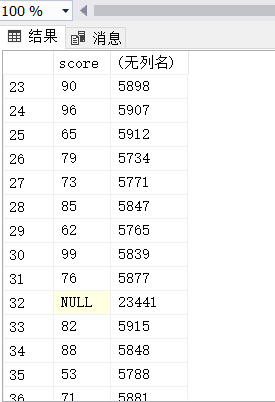
\includegraphics[width=0.9\textwidth]{fig32.png}
\end{subfigure}
\begin{subfigure}{0.3\textwidth}
  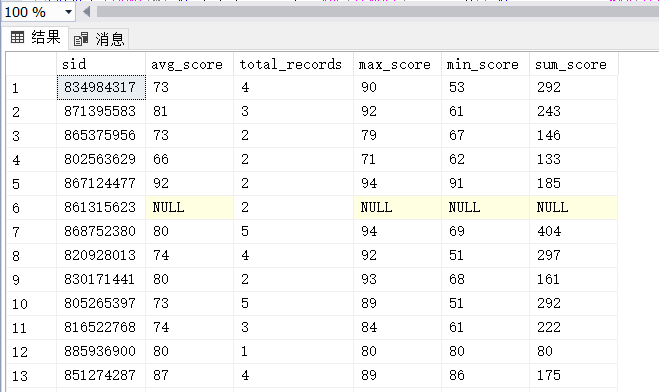
\includegraphics[width=0.9\textwidth]{fig33.png}
\end{subfigure}
\end{figure}

\item 查询成绩小于60的选课记录,统计总数、平均分、最大值和最小值。
\begin{quote}
\texttt{
SELECT COUNT(*) AS total\_records, AVG(ISNULL(score, 0)) AS avg\_score, MAX(ISNULL(score, 0)) AS max\_score, MIN(ISNULL(score, 0)) AS min\_score
FROM CHOICES
WHERE ISNULL(score, 0) < 60;
}
\end{quote}

\item 采用嵌套查询的方式,利用比较运算符和谓词ALL的结合来查询表COURSES中最少的课时。假设数据库中只有一个记录的时候,使用前面的方法会得到什么结果,为什么?
\begin{quote}
\texttt{
SELECT MIN(hour) FROM COURSES WHERE hour <= ALL (SELECT hour FROM COURSES WHERE hour > 0);
}
\end{quote}

如果数据库中只有一个记录,那么子查询\texttt{SELECT hour FROM COURSES}将返回该记录的课时,
并且它是该表课时的最小值。因此,主查询中WHERE子句的条件
\texttt{hour >= ALL(SELECT hour FROM COURSES)}也将成立,
因此查询结果将为该记录的课时值。


\begin{figure}[h]
\centering
\caption{运行结果}
\begin{subfigure}{0.3\textwidth}
  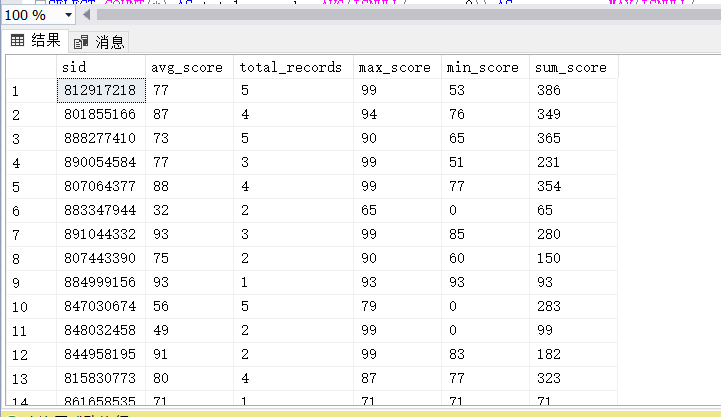
\includegraphics[width=0.9\textwidth]{fig34.png}
\end{subfigure}
\begin{subfigure}{0.3\textwidth}
  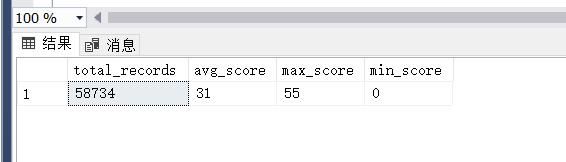
\includegraphics[width=0.9\textwidth]{fig35.png}
\end{subfigure}
\end{figure}

\item 创建一个学生表\texttt{S(NO,  SID,  SNAME)}, 教师表\texttt{T(NO,  TID,  TNAME)}作为实验用的表。其中NO分别是这两个表的主键, 其他键允许为空。
向S插入元组\texttt{(1,  0129871001,  王小明)}、\texttt{(2,  0129871002,  李兰)}、\texttt{(3,  0129871005,  NULL)}、\texttt{(4,  0129871004,  关红)};
向T插入元组\texttt{(1,  100189,  王小明)}、\texttt{(2,  100180,  李小)}、\texttt{(3,  100121,  NULL)}、\texttt{(4,  100128,  NULL)}。
对这两个表作对姓名的等值连接运算, 找出既是老师又是学生的人员的学生编号和老师编号。 
\begin{quote}
\texttt{
CREATE TABLE S (
    NO INT PRIMARY KEY,
    SID CHAR(10),
    SNAME VARCHAR(20)
);
\\
CREATE TABLE T (
    NO INT PRIMARY KEY,
    TID CHAR(10),
    TNAME VARCHAR(20)
);
}
\end{quote}
\begin{quote}
\texttt{
INSERT INTO S(NO, SID, SNAME) VALUES
(1, '0129871001', '王小明'),
(2, '0129871002', '李兰'),
(3, '0129871005', NULL),
(4, '0129871004', '关红');
\\
INSERT INTO T(NO, TID, TNAME) VALUES
(1, '100189', '王小明'),
(2, '100180', '李小'),
(3, '100121', NULL),
(4, '100128', NULL);
\\
SELECT * FROM S
\\
SELECT * FROM T
}
\end{quote}
\begin{quote}
\texttt{
SELECT S.SID, T.TID
FROM S JOIN T ON S.SNAME = T.TNAME
WHERE S.SNAME IS NOT NULL AND T.TNAME IS NOT NULL;
}
\end{quote}


\begin{figure}[h]
\centering
\caption{运行结果}
\begin{subfigure}{0.3\textwidth}
  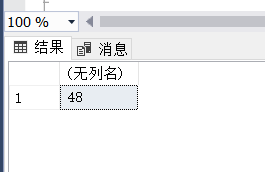
\includegraphics[width=0.9\textwidth]{fig36.png}
\end{subfigure}
\begin{subfigure}{0.3\textwidth}
  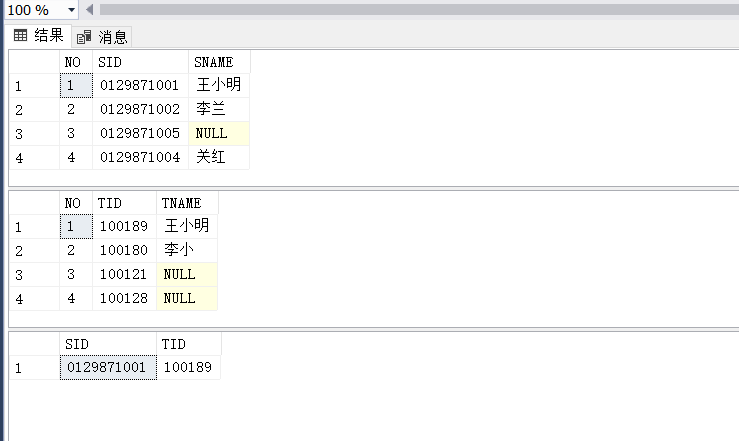
\includegraphics[width=0.9\textwidth]{fig37.png}
\end{subfigure}
\end{figure}

\end{enumerate}

\end{spacing}

\end{document}